\chapter{Additional distance plots}
\label{sec:additional_distances}

\begin{figure}[t]
    \centering
    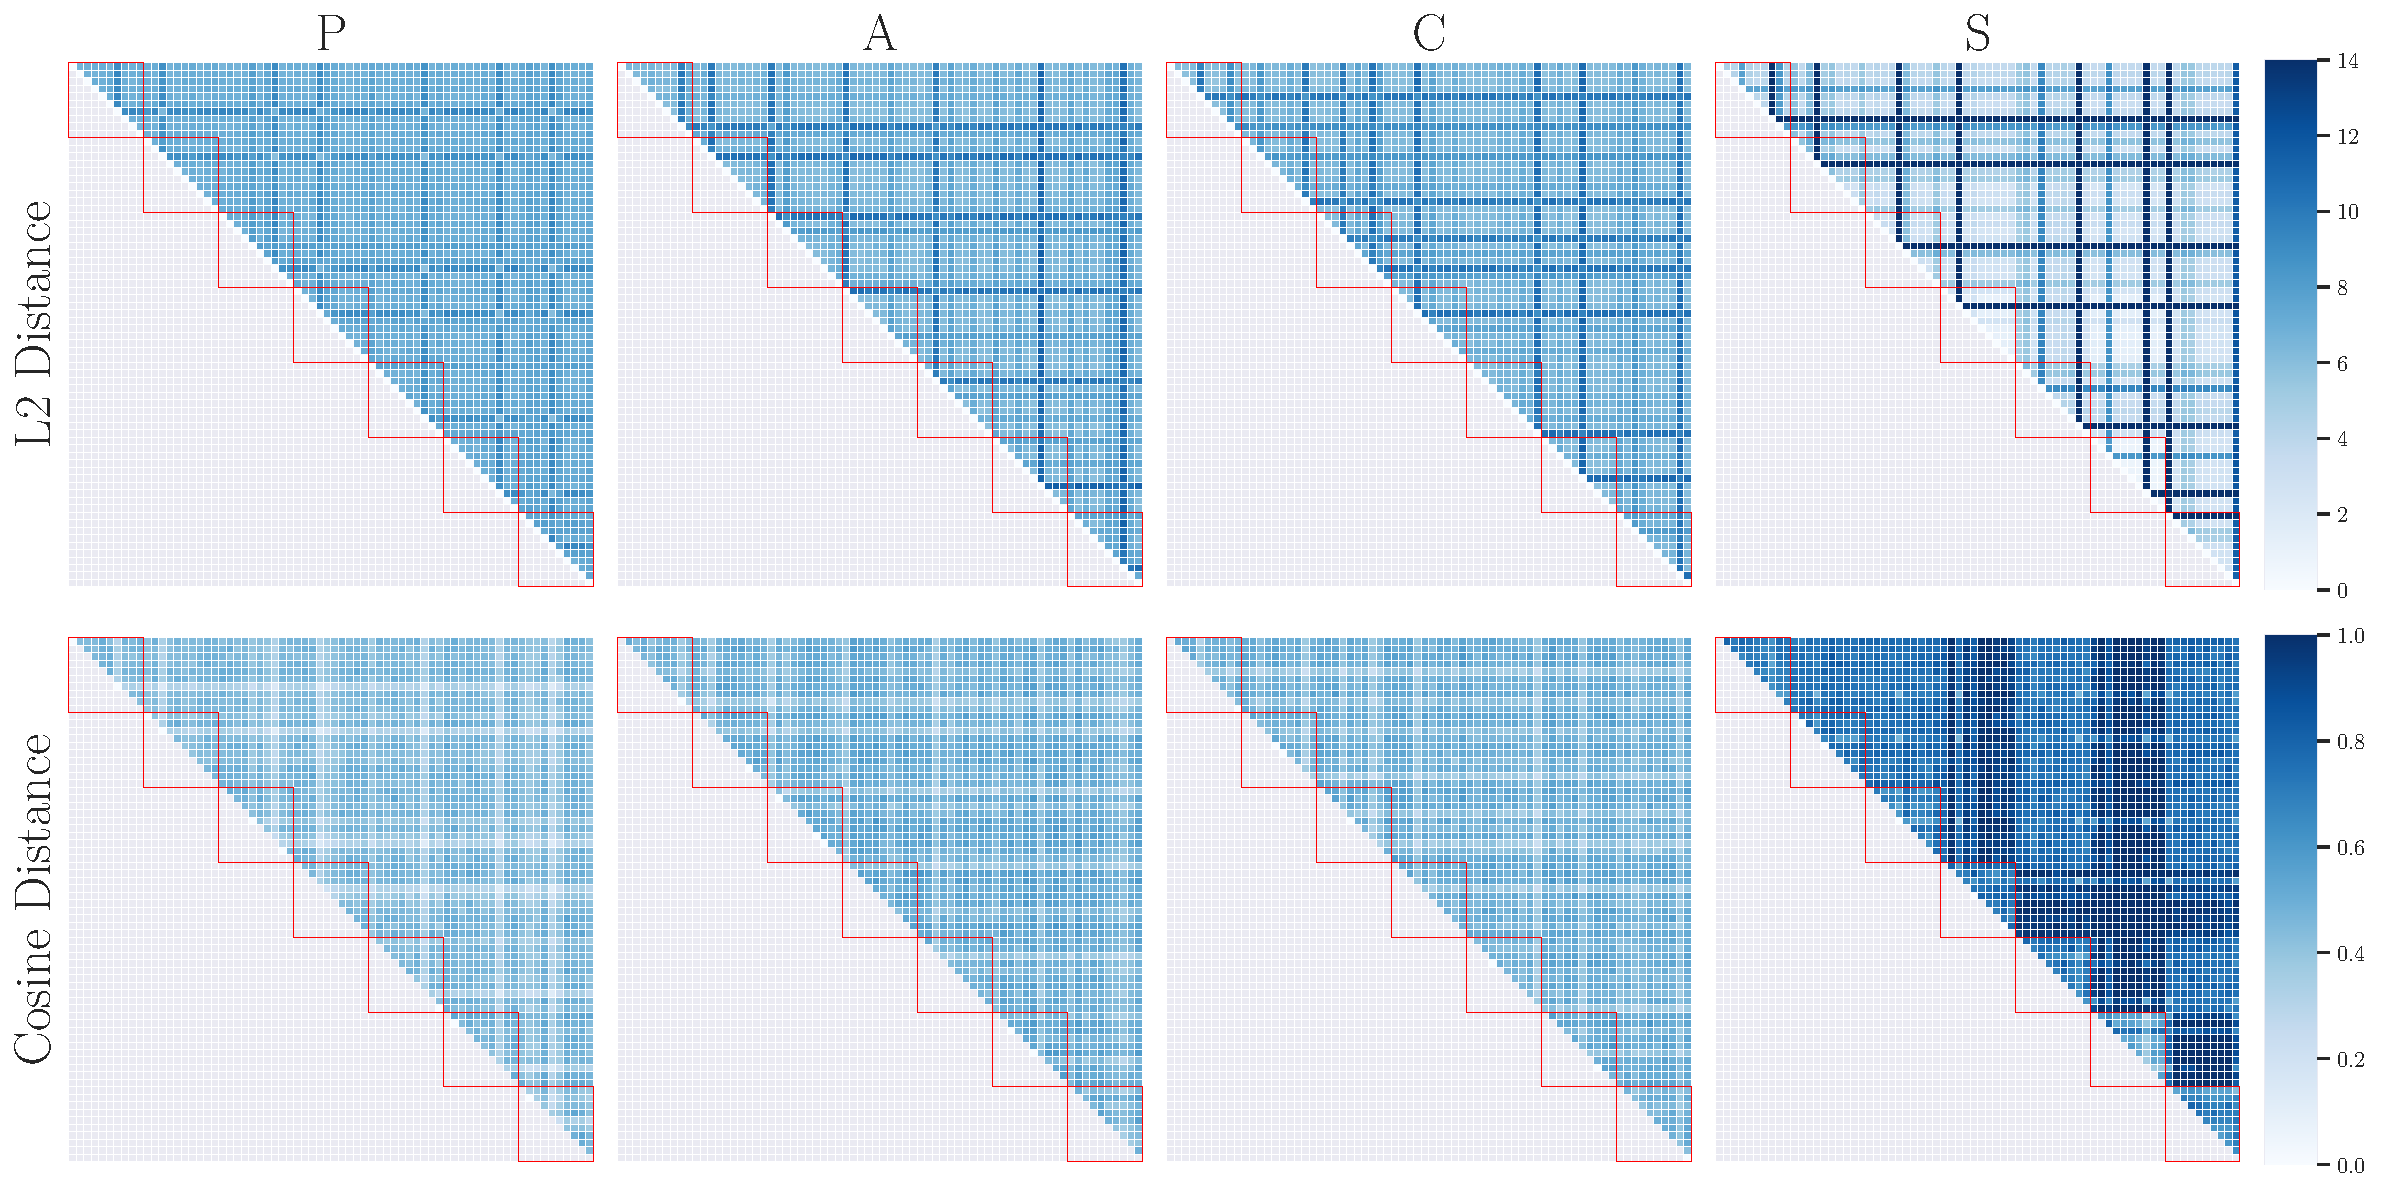
\includegraphics[width=\textwidth]{Figures/Chapter4/2021-01-21-ProDropIncorrectWeight-1.0SAVEResNet18oracle_validation_trial0.pdf}
    \caption[First data split pairwise prototype distances with $w_{c,j} = 0.0$] {Best-performing pairwise learned prototype $\ell_2$-distance (top) and cosine distance $\cdistance$ (bottom) with negative weight $w_{c,j} = -1.0\; \forall j: \prot \notin \prots_c$ for each testing domain. Red squares denote prototype class correspondence for the $7$ different classes in the PACS dataset. No self-challenging is applied and colormap bounds are adjusted per metric for visualization purposes. First data split.}
    \label{fig:pairwise_distance}
\end{figure}

\begin{figure}[h]
    \centering
    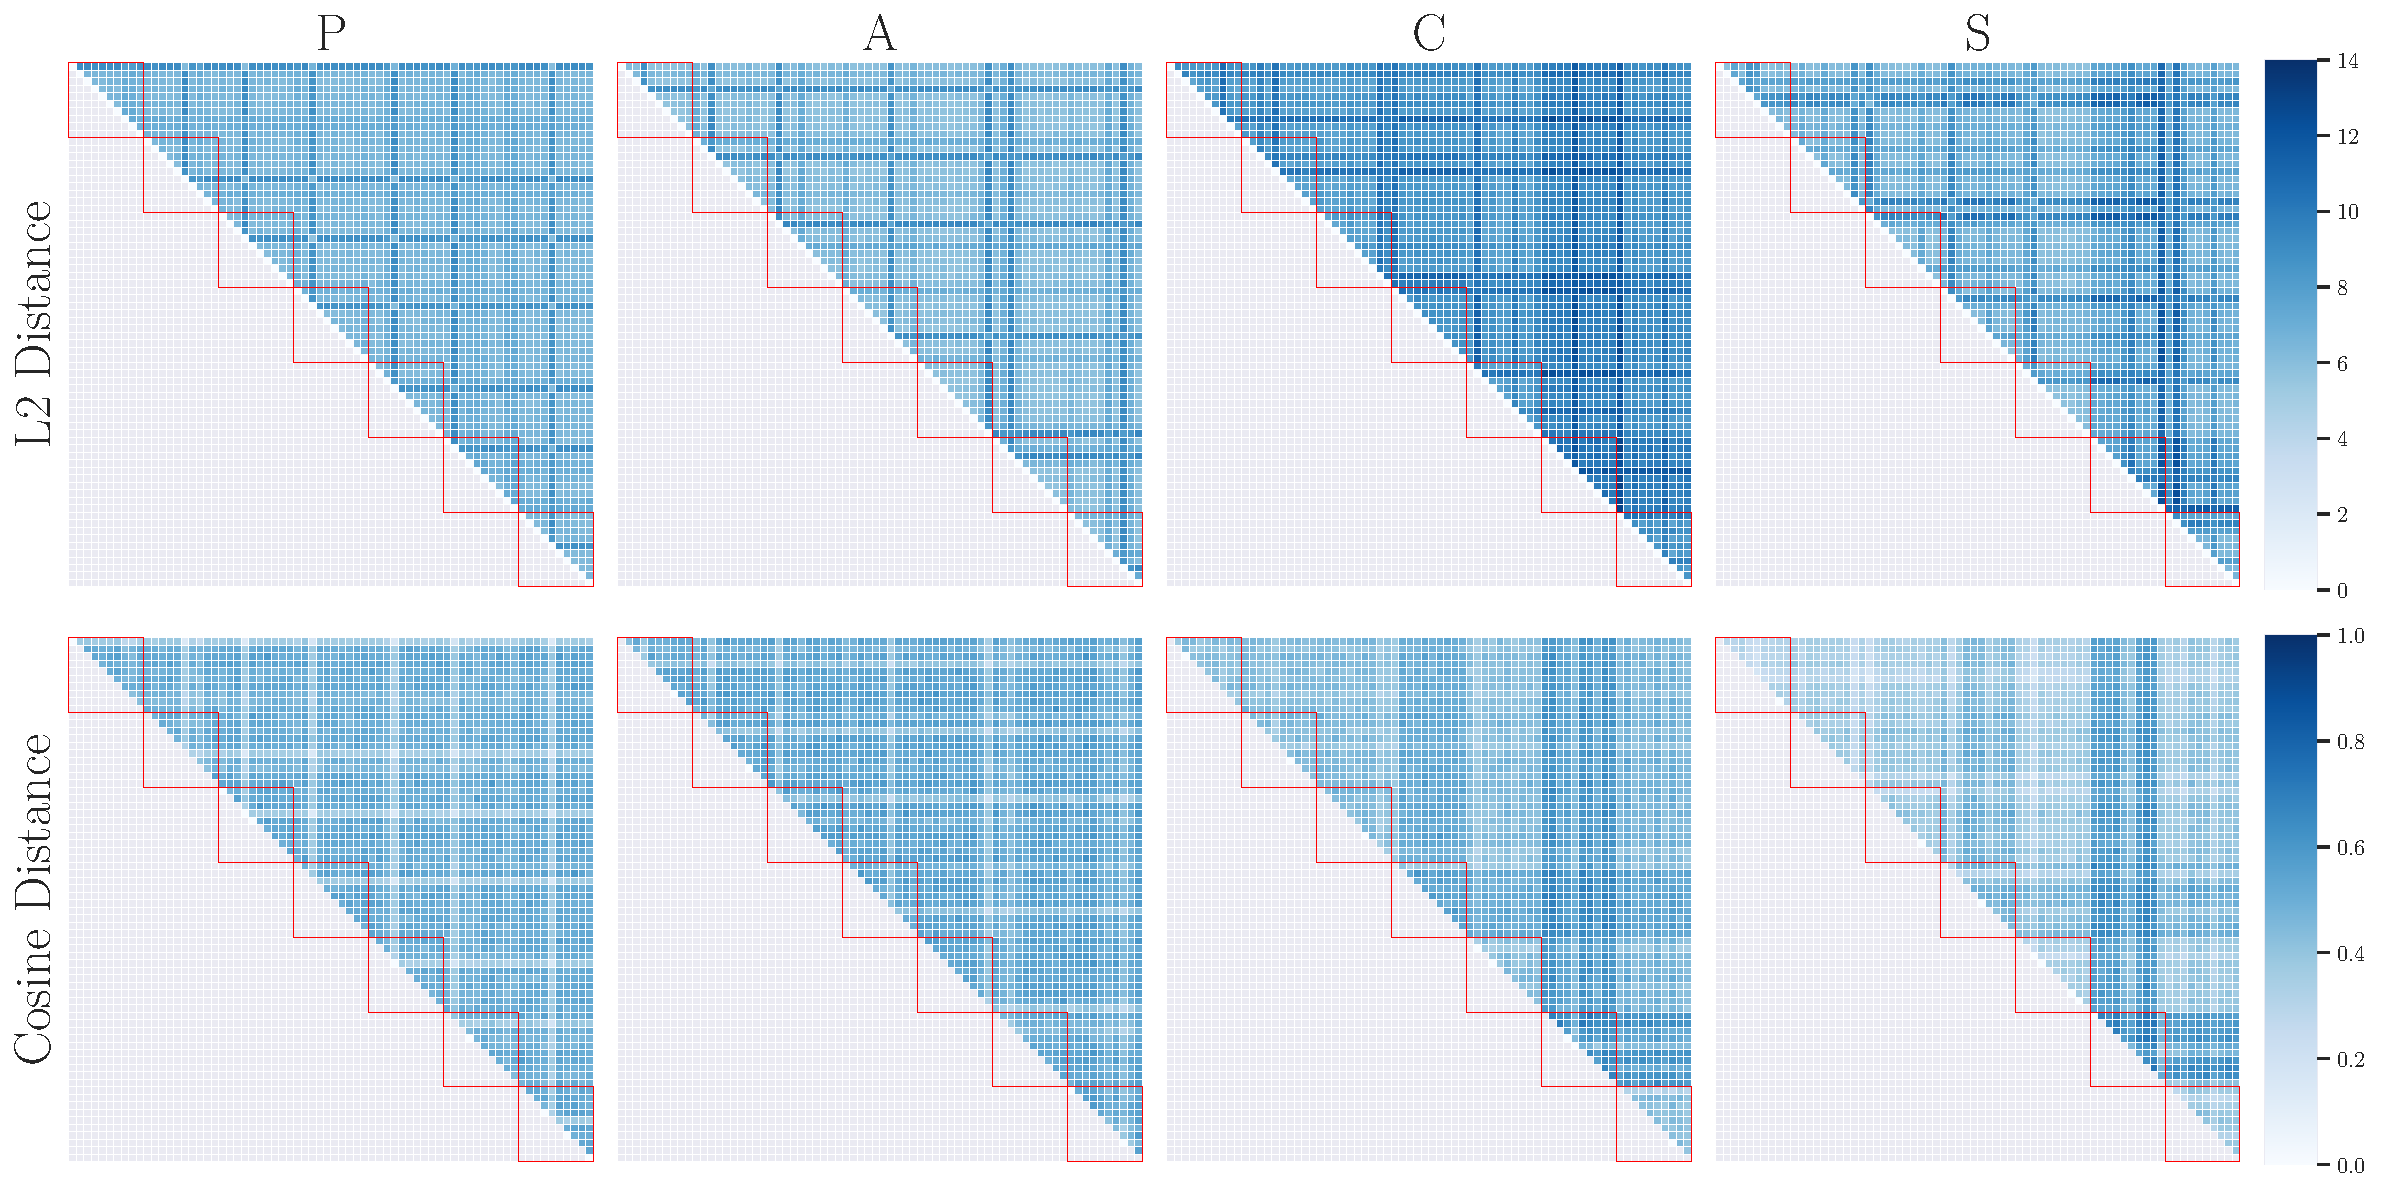
\includegraphics[width=\textwidth]{Figures/Chapter4/2021-01-21-ProDropIncorrectWeight-1.0SAVEResNet18oracle_validation_trial2.pdf}
    \caption[Third data split pairwise prototype distances with $w_{c,j} = -1.0$] {Best-performing pairwise learned prototype $\ell_2$-distance (top) and cosine distance $\cdistance$ (bottom) with negative weight $w_{c,j} = -1.0\; \forall j: \prot \notin \prots_c$ for each testing domain. Red squares denote prototype class correspondence for the $7$ different classes in the PACS dataset. No self-challenging is applied and colormap bounds are adjusted per metric for visualization purposes. Third data split.}
    \label{fig:pw_distance_trial2}
\end{figure}

\begin{figure}[t]
    \centering
    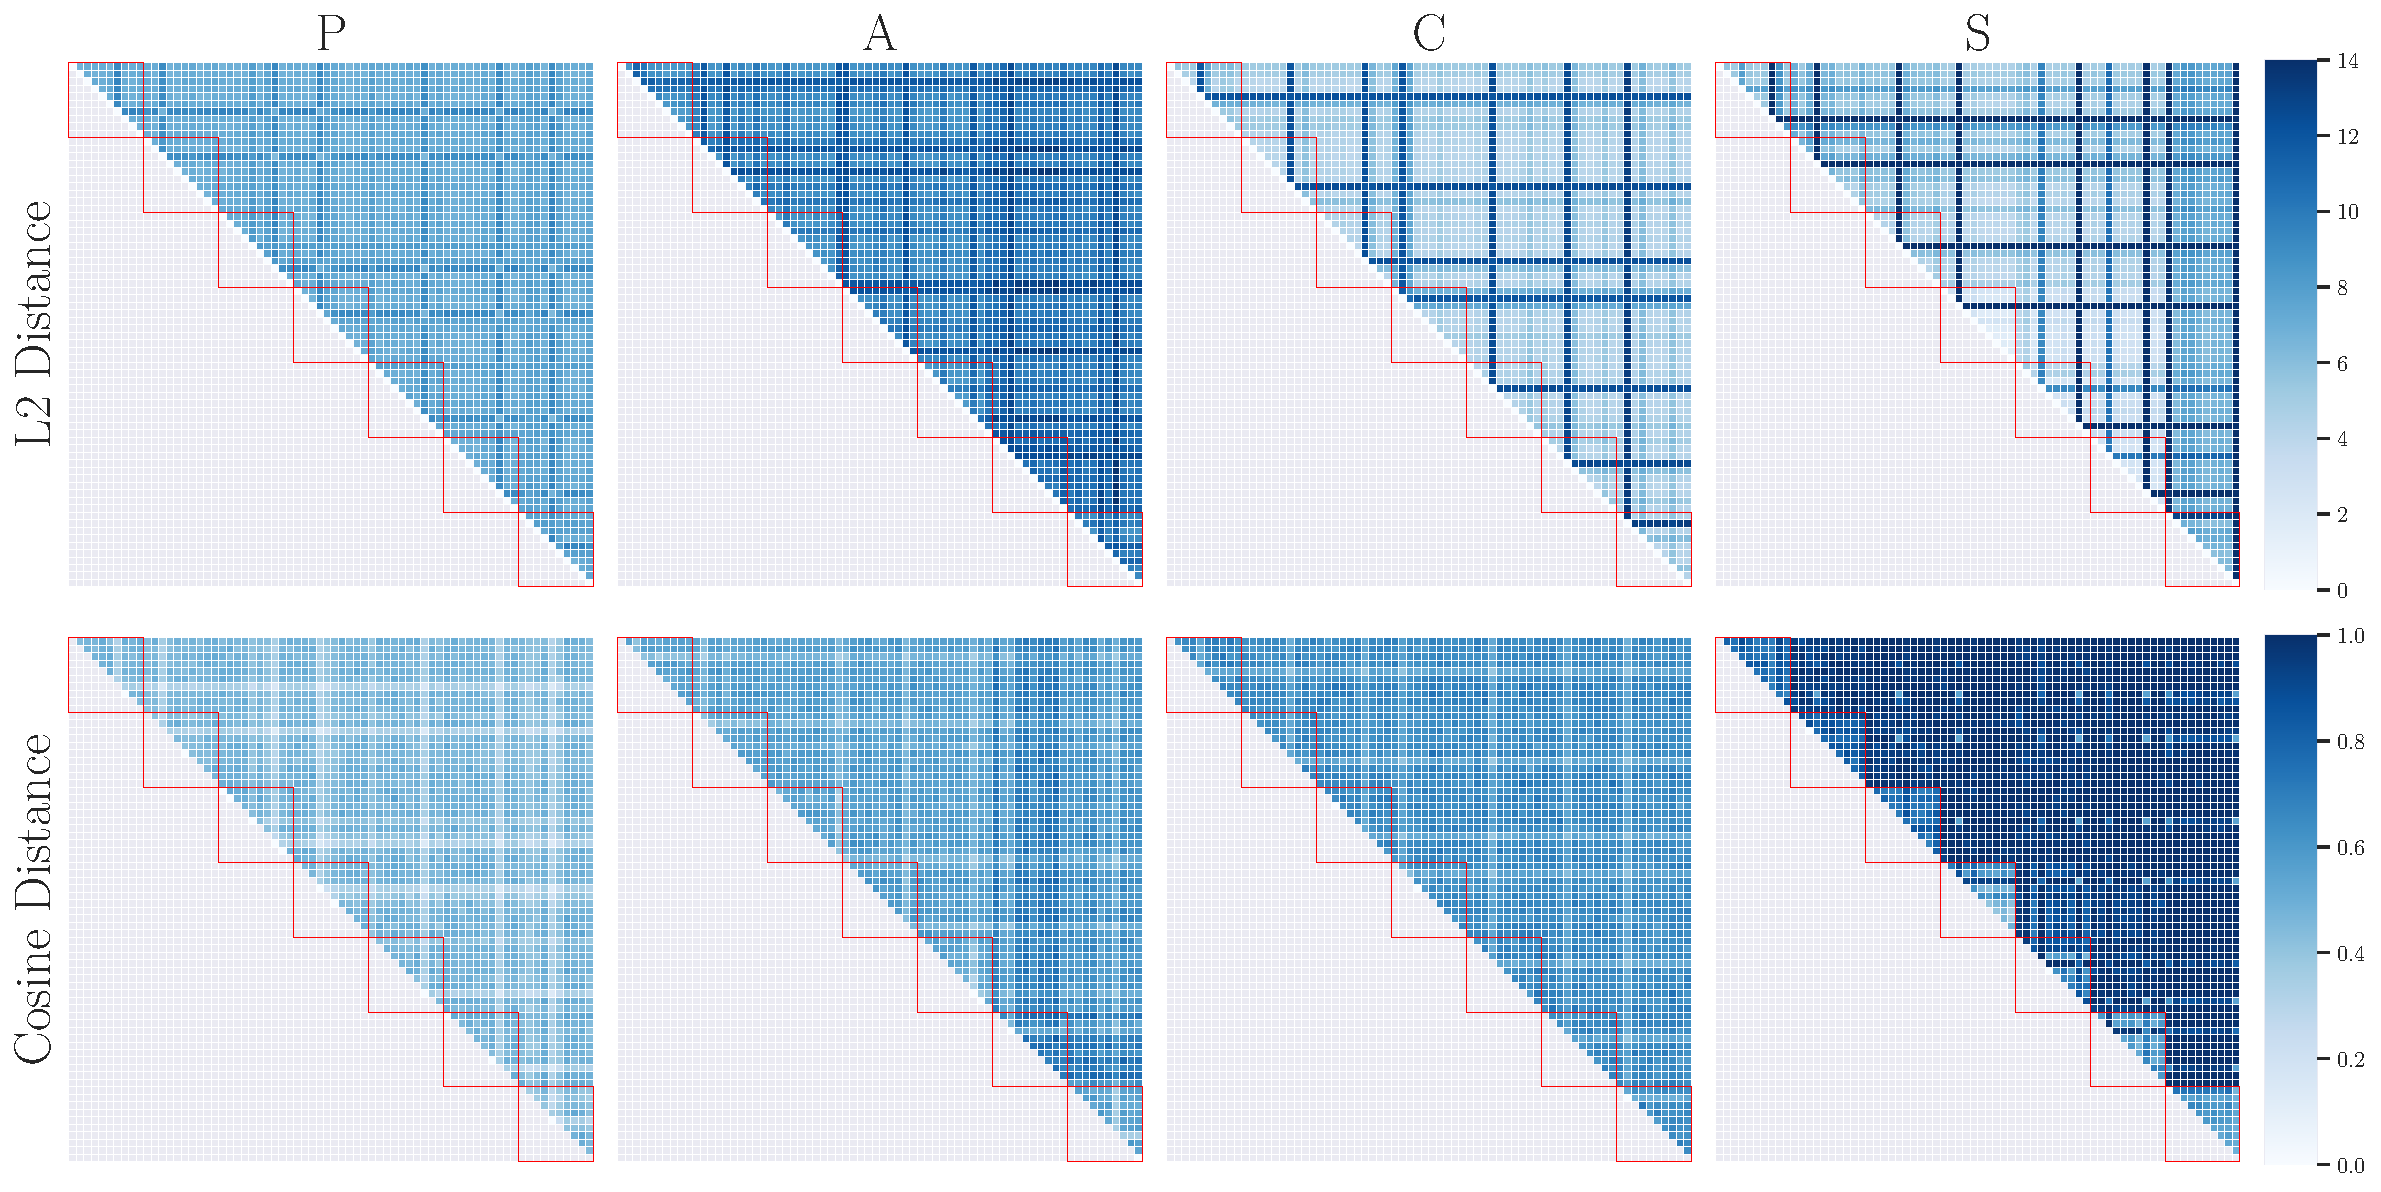
\includegraphics[width=\textwidth]{Figures/Chapter4/2021-01-21-ProDropIncorrectWeight-1.0WithSCdrop_f0.5SAVEResNet18oracle_validation_trial0.pdf}
    \caption[First data split pairwise self-challenging prototype distances with $w_{c,j} = -1.0$] {Best-performing pairwise learned prototype $\ell_2$-distance (top) and cosine distance $\cdistance$ (bottom) with negative weight $w_{c,j} = -1.0\; \forall j: \prot \notin \prots_c$ for each testing domain. Red squares denote prototype class correspondence for the $7$ different classes in the PACS dataset. Self-challenging is applied and colormap bounds are adjusted per metric for visualization purposes. First data split.}
    \label{fig:pairwise_distance_sc}
\end{figure}

\begin{figure}[h]
    \centering
    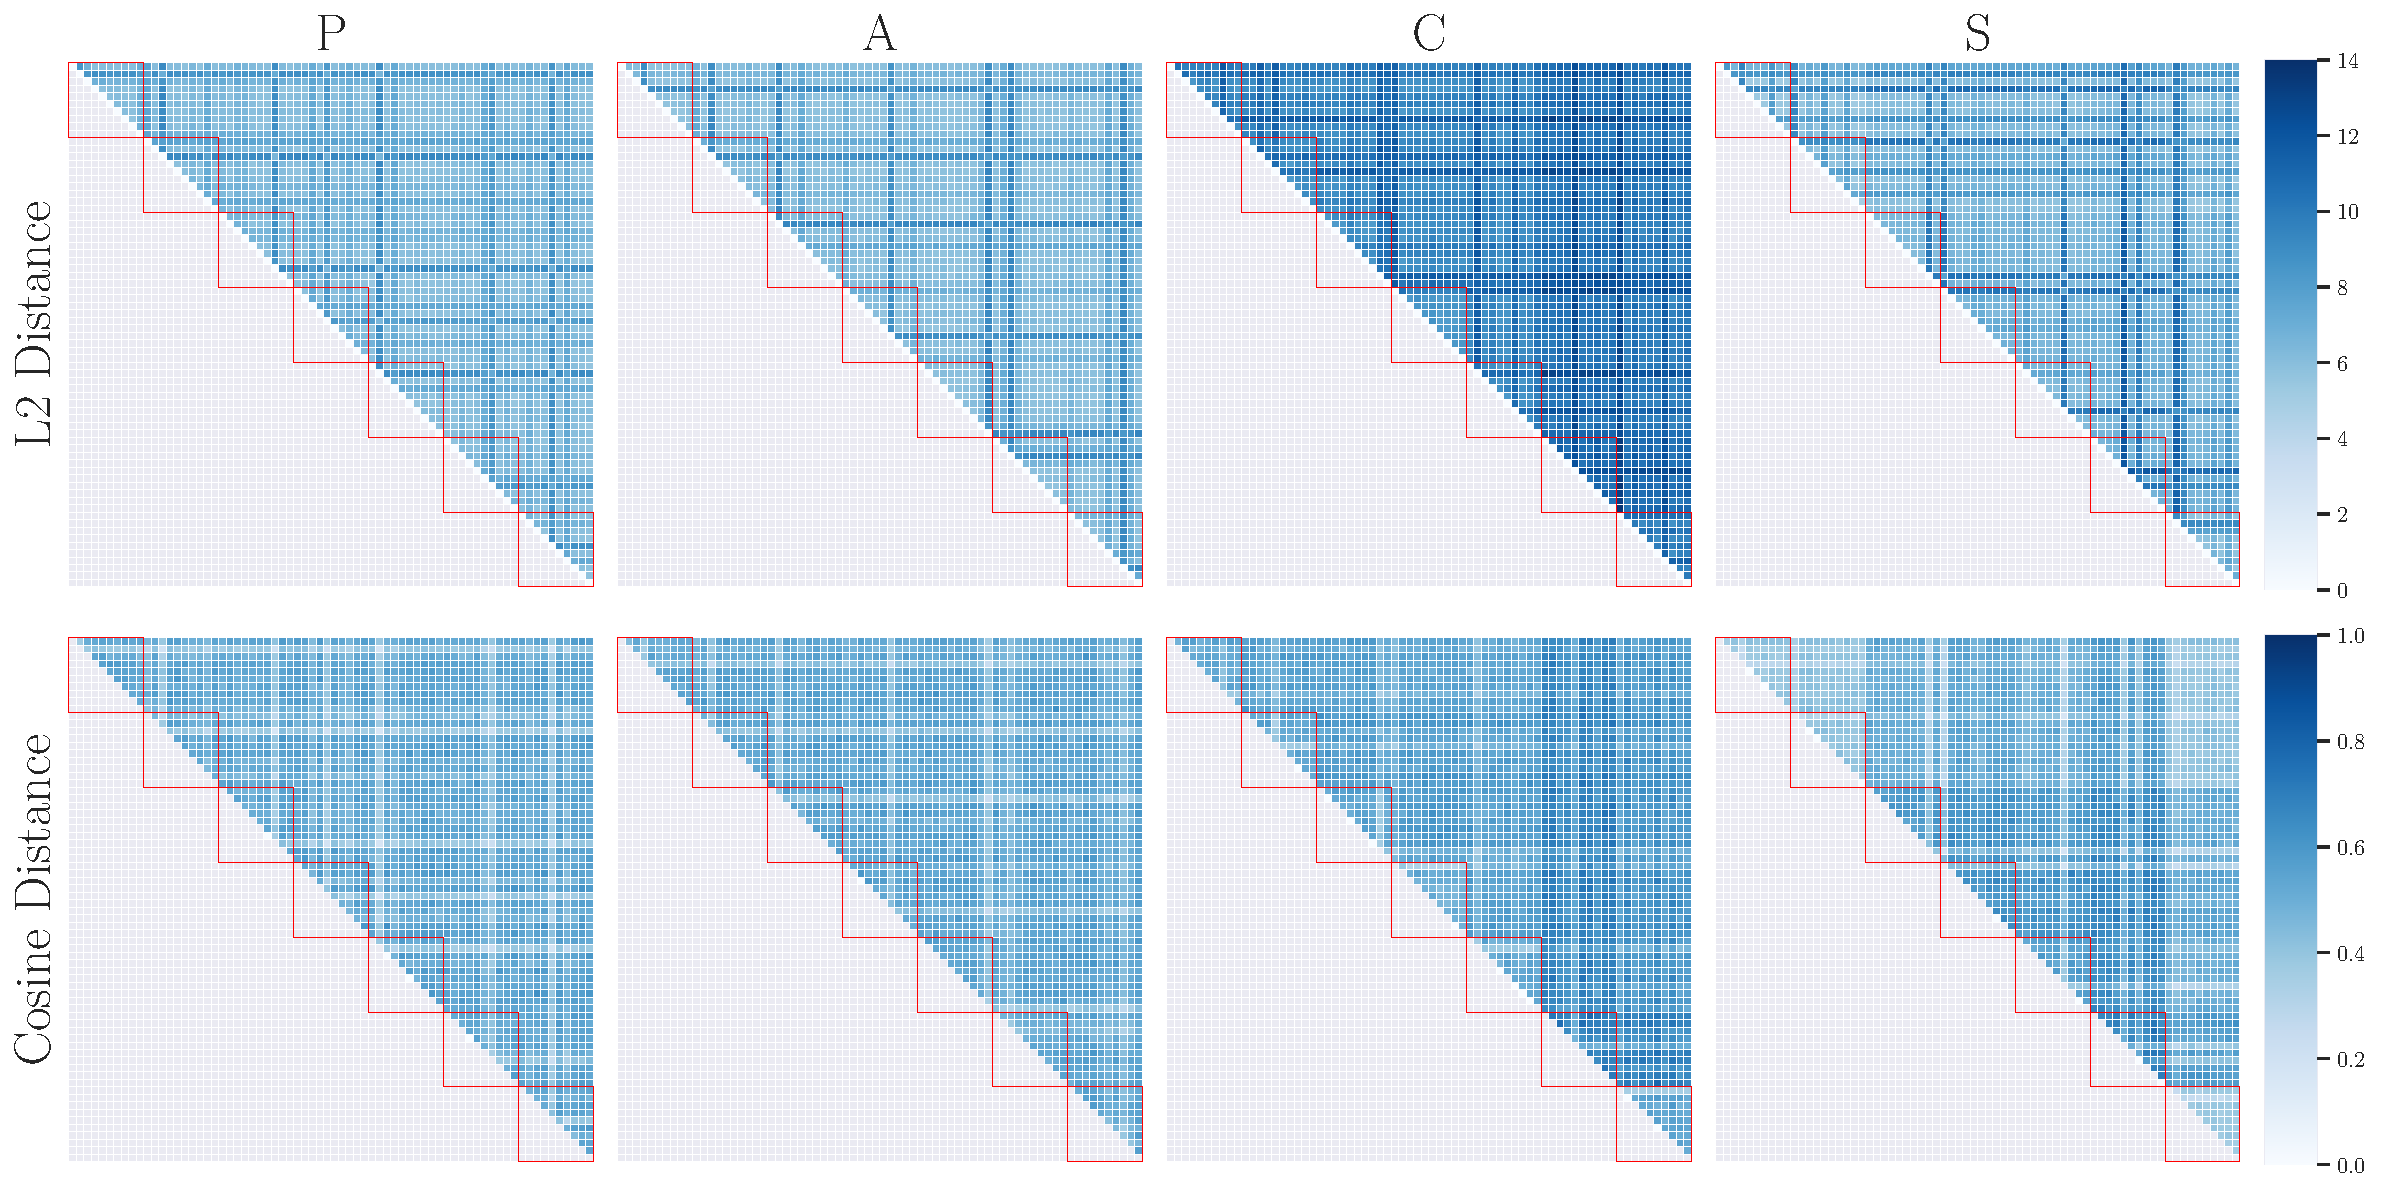
\includegraphics[width=\textwidth]{Figures/Chapter4/2021-01-21-ProDropIncorrectWeight-1.0WithSCdrop_f0.5SAVEResNet18oracle_validation_trial2.pdf}
    \caption[Third data split pairwise self-challenging prototype distances with $w_{c,j} = -1.0$] {Best-performing pairwise learned prototype $\ell_2$-distance (top) and cosine distance $\cdistance$ (bottom) with negative weight $w_{c,j} = -1.0\; \forall j: \prot \notin \prots_c$ for each testing domain. Red squares denote prototype class correspondence for the $7$ different classes in the PACS dataset. Self-challenging is applied and colormap bounds are adjusted per metric for visualization purposes. Third data split.}
\end{figure}


%%%%%

\begin{figure}[h]
    \centering
    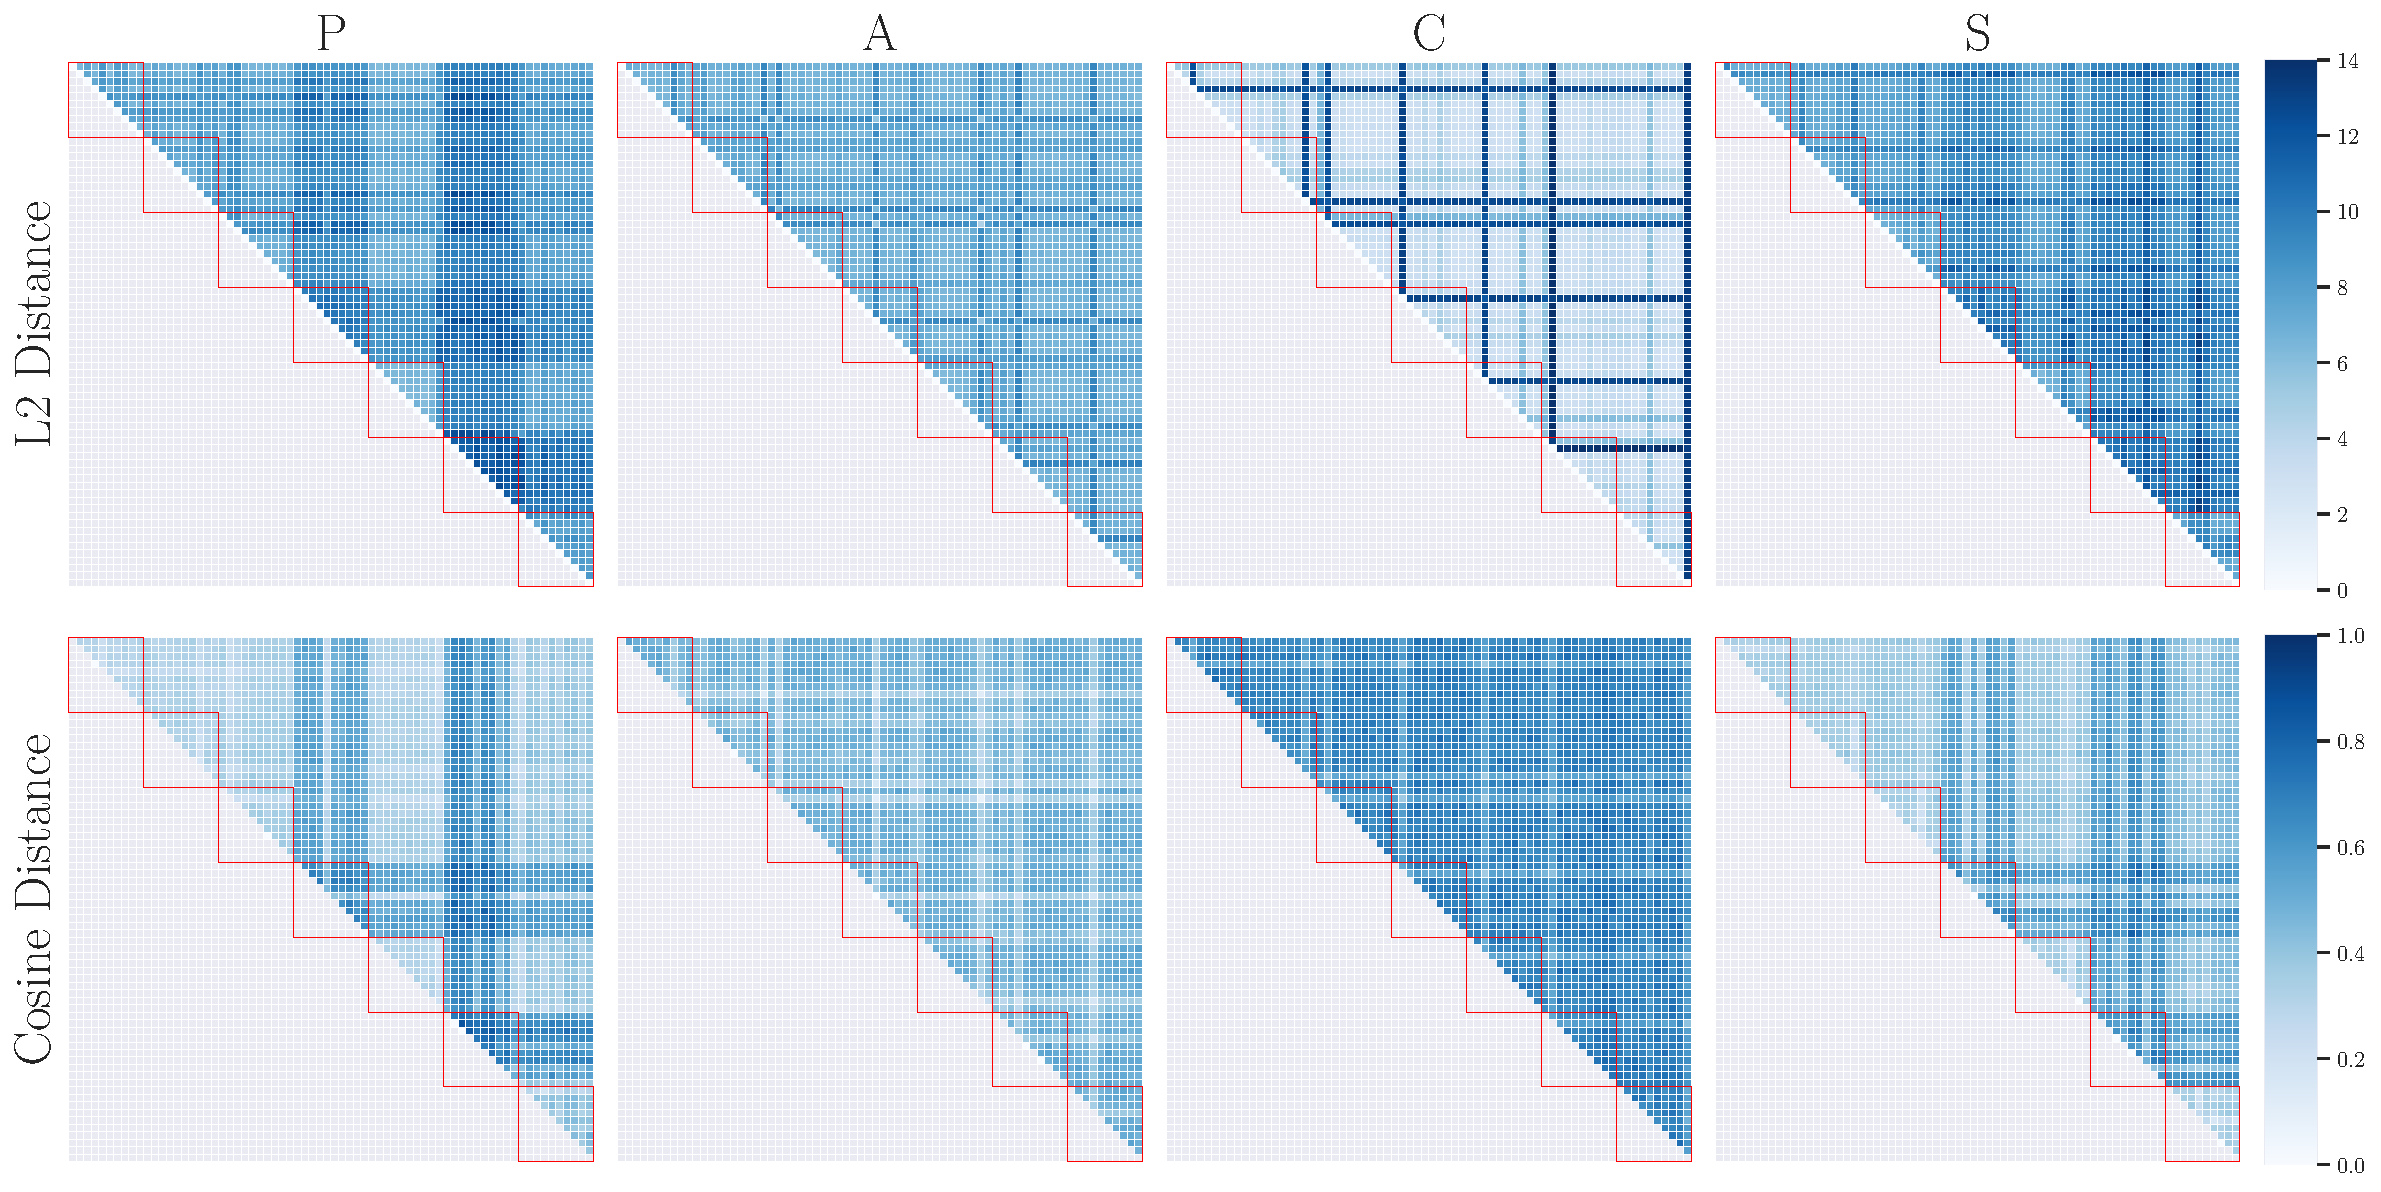
\includegraphics[width=\textwidth]{Figures/Chapter4/2021-01-21-ProDropIncorrectWeight0.0SAVEResNet18oracle_validation_trial1.pdf}
    \caption[Second data split pairwise prototype distances with $w_{c,j} = 0.0$] {Best-performing pairwise learned prototype $\ell_2$-distance (top) and cosine distance $\cdistance$ (bottom) with negative weight $w_{c,j} = 0.0\; \forall j: \prot \notin \prots_c$ for each testing domain. Red squares denote prototype class correspondence for the $7$ different classes in the PACS dataset. No self-challenging is applied and colormap bounds are adjusted per metric for visualization purposes. Second data split.}
    \label{fig:pw_distance_0.0_trial1}
\end{figure}

\begin{figure}[h]
    \centering
    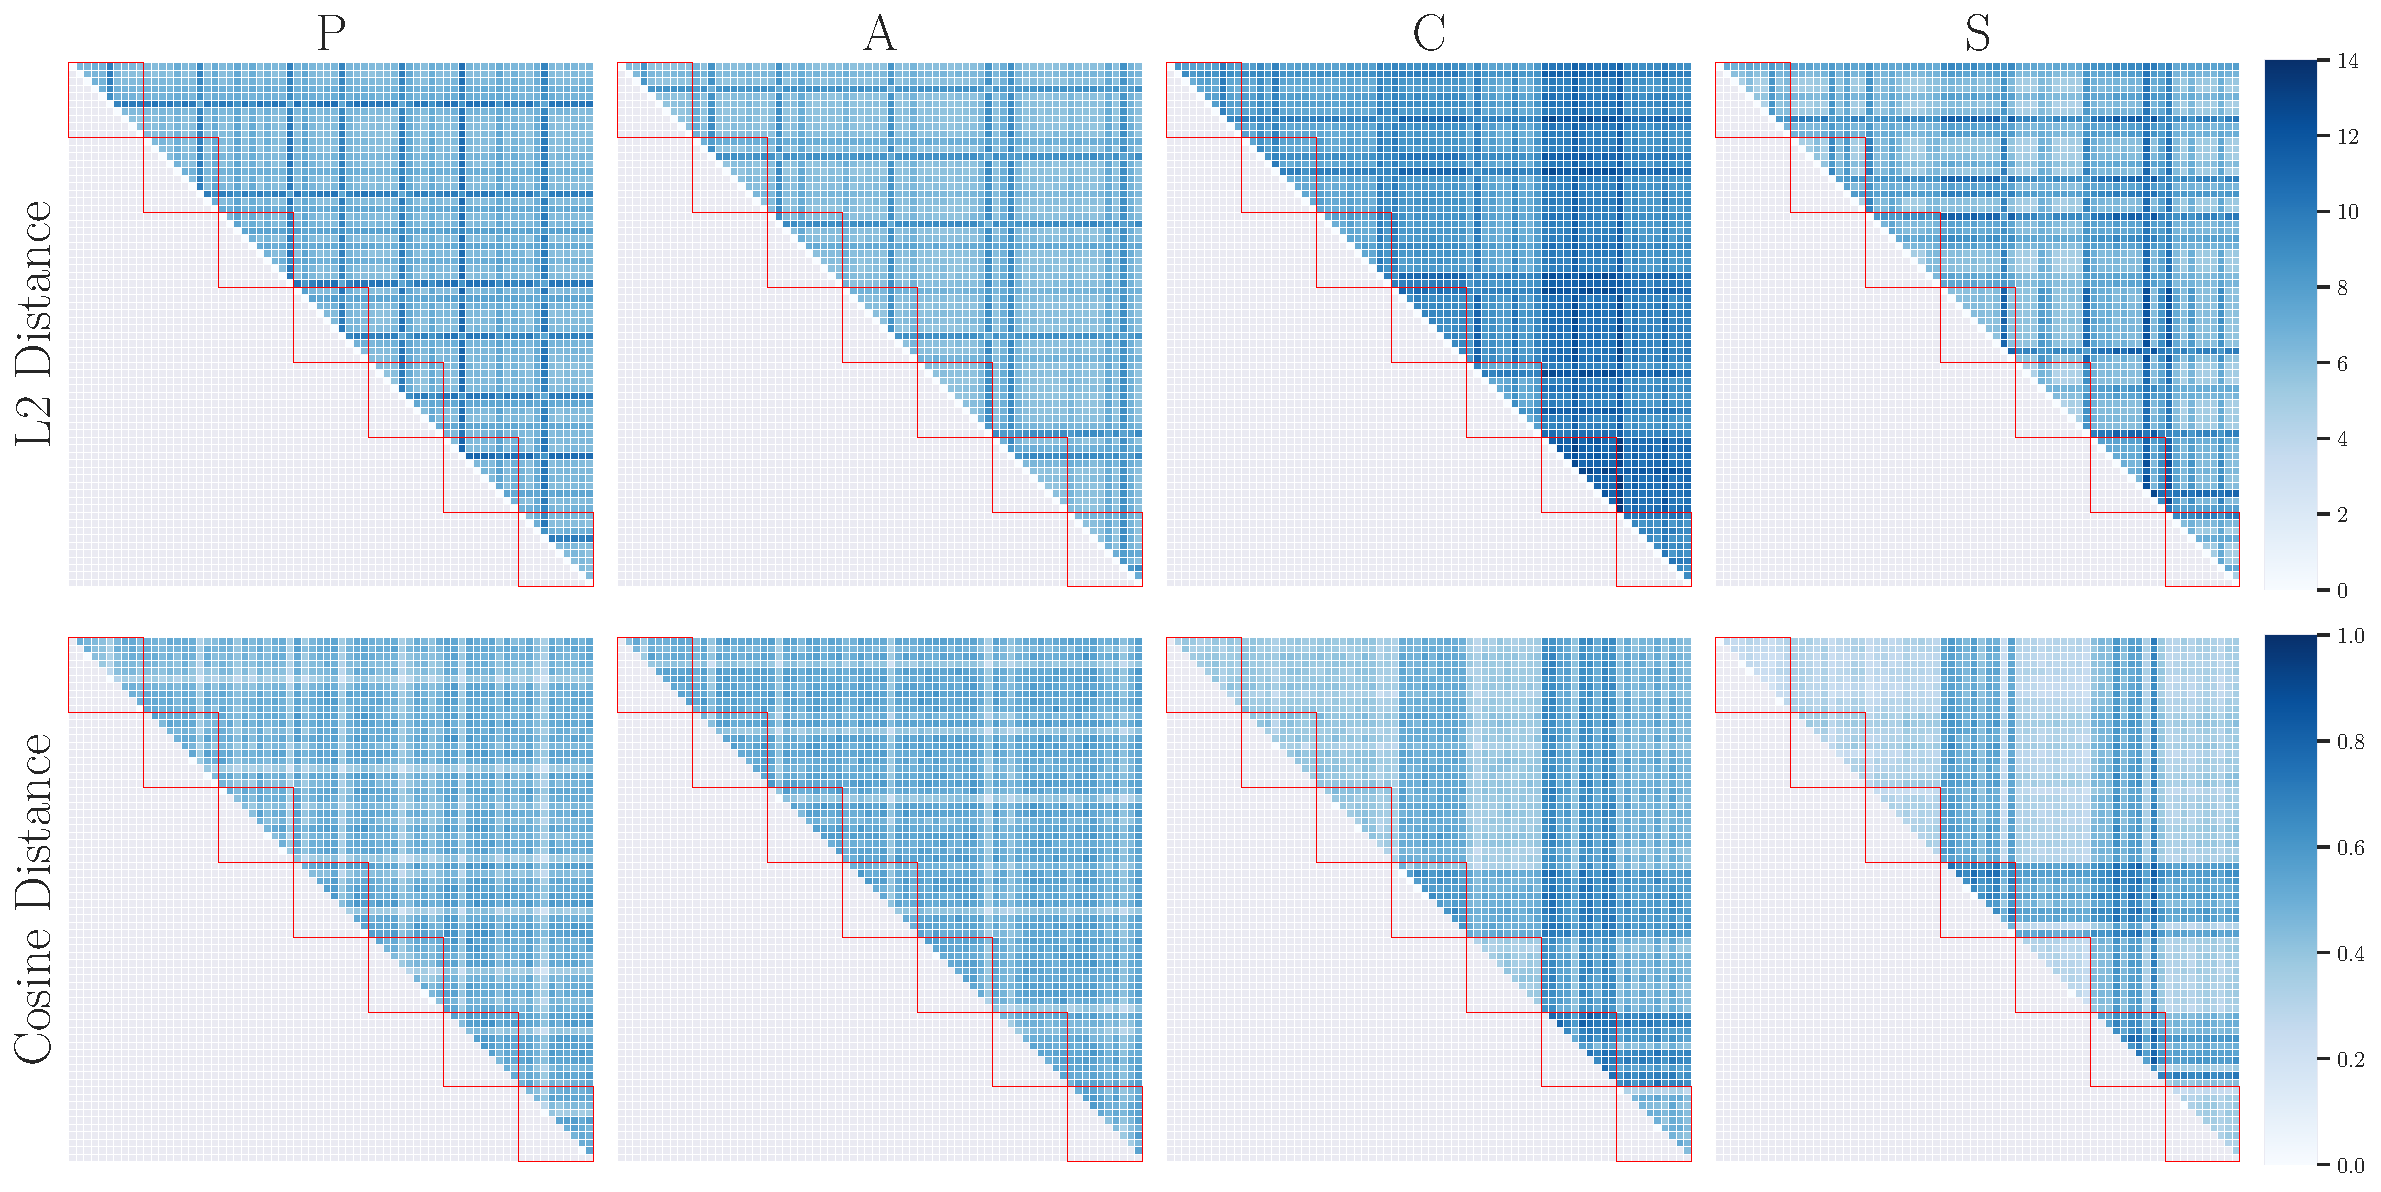
\includegraphics[width=\textwidth]{Figures/Chapter4/2021-01-21-ProDropIncorrectWeight0.0SAVEResNet18oracle_validation_trial2.pdf}
    \caption[Third data split pairwise prototype distances with $w_{c,j} = 0.0$] {Best-performing pairwise learned prototype $\ell_2$-distance (top) and cosine distance $\cdistance$ (bottom) with negative weight $w_{c,j} = 0.0\; \forall j: \prot \notin \prots_c$ for each testing domain. Red squares denote prototype class correspondence for the $7$ different classes in the PACS dataset. No self-challenging is applied and colormap bounds are adjusted per metric for visualization purposes. Third data split.}
    \label{fig:pw_distance_0.0_trial2}
\end{figure}

\begin{figure}[h]
    \centering
    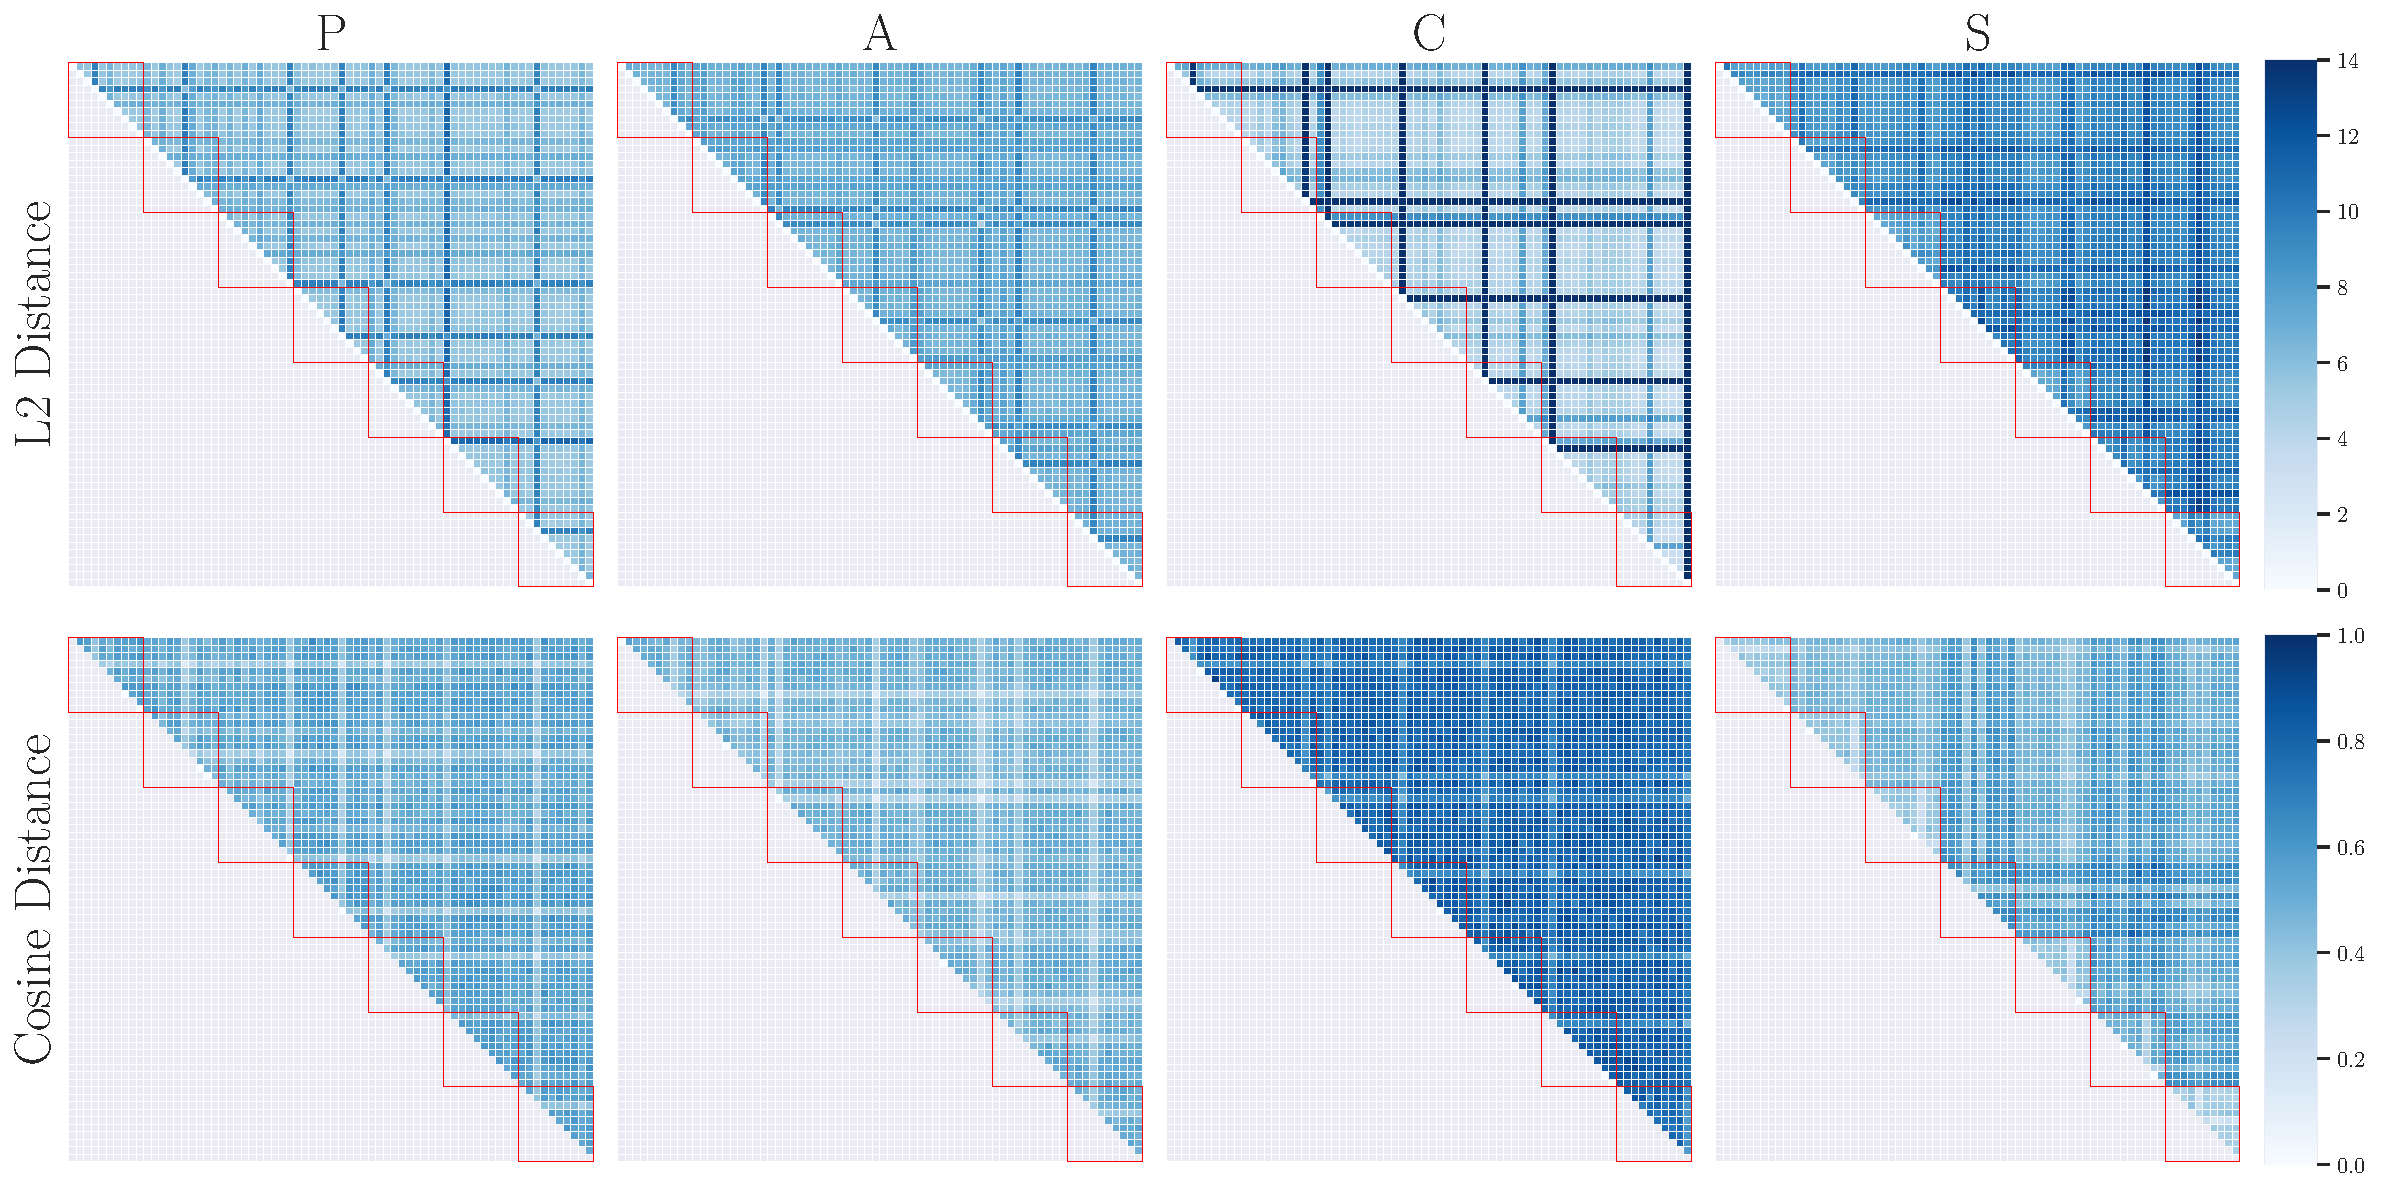
\includegraphics[width=\textwidth]{Figures/Chapter4/2021-01-21-ProDropIncorrectWeight0.0WithSCdrop_f0.5SAVEResNet18oracle_validation_trial1.pdf}
    \caption[Second data split pairwise self-challenging prototype distances with $w_{c,j} = 0.0$] {Best-performing pairwise learned prototype $\ell_2$-distance (top) and cosine distance $\cdistance$ (bottom) with negative weight $w_{c,j} = 0.0\; \forall j: \prot \notin \prots_c$ for each testing domain. Red squares denote prototype class correspondence for the $7$ different classes in the PACS dataset. Self-challenging is applied and colormap bounds are adjusted per metric for visualization purposes. Second data split.}
    \label{fig:pw_distance_0.0_trial1-sc}
\end{figure}

\begin{figure}[h]
    \centering
    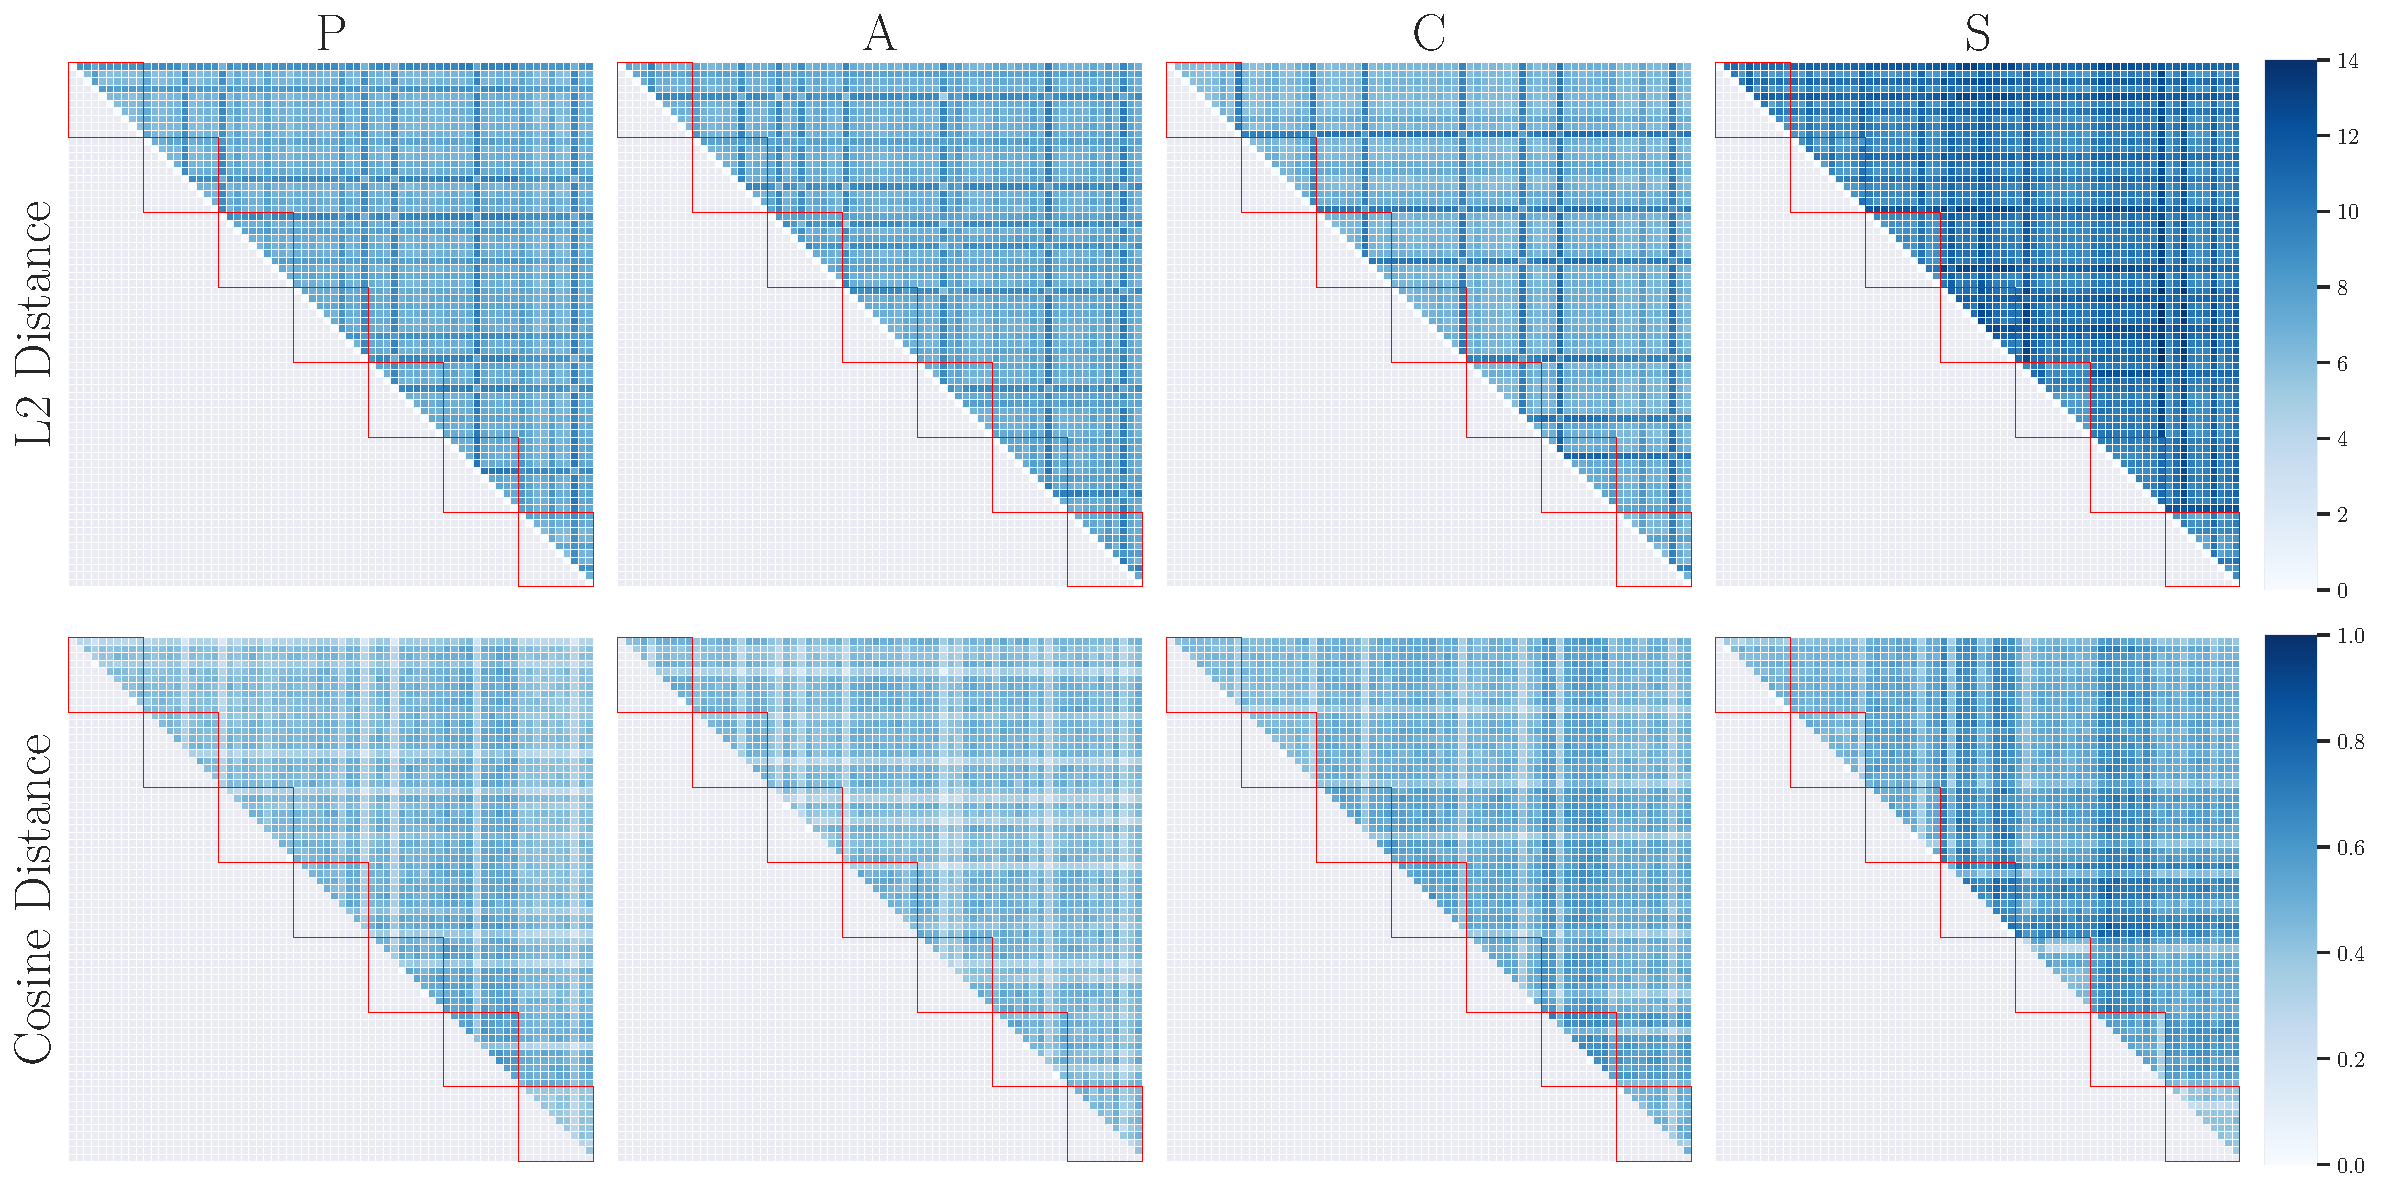
\includegraphics[width=\textwidth]{Figures/Chapter4/2021-01-21-ProDropIncorrectWeight0.0WithSCdrop_f0.5SAVEResNet18oracle_validation_trial2.pdf}
    \caption[Third data split pairwise self-challenging prototype distances with $w_{c,j} = 0.0$] {Best-performing pairwise learned prototype $\ell_2$-distance (top) and cosine distance $\cdistance$ (bottom) with negative weight $w_{c,j} = 0.0\; \forall j: \prot \notin \prots_c$ for each testing domain. Red squares denote prototype class correspondence for the $7$ different classes in the PACS dataset. Self-challenging is applied and colormap bounds are adjusted per metric for visualization purposes. Third data split.}
    \label{fig:pw_distance_0.0_trial2-sc}
\end{figure}